\documentclass[aspectratio=169]{beamer}
\usepackage[T1]{fontenc}
\usepackage[utf8]{inputenc}
\usepackage{lmodern}
\usepackage{microtype}
\usepackage{xcolor}
\usepackage{tikz}
\usetikzlibrary{positioning, arrows.meta}
\usepackage{fontawesome5}

\definecolor{wurgreen}{HTML}{34B233}
\definecolor{darkgreen}{HTML}{1F6B1E}
\definecolor{darknavy}{HTML}{1A1A2E}
\definecolor{midgray}{HTML}{6B7280}
\definecolor{lightgray}{HTML}{F3F4F6}
\definecolor{lightgreen}{HTML}{E8F7E8}
\definecolor{bodytext}{HTML}{1F2937}
\definecolor{warnred}{HTML}{FEE2E2}
\definecolor{warnborder}{HTML}{EF4444}

\usetheme{default}
\usecolortheme{default}
\usefonttheme{professionalfonts}
\setbeamertemplate{navigation symbols}{}
\setbeamertemplate{itemize items}{\textcolor{wurgreen}{\textbullet}}
\setbeamertemplate{itemize subitem}{\textcolor{midgray}{--}}
\setbeamercolor{frametitle}{fg=white, bg=darknavy}
\setbeamerfont{frametitle}{size=\large, series=\bfseries}
\setbeamertemplate{frametitle}{%
  \begin{beamercolorbox}[wd=\paperwidth, ht=1.1cm, dp=0.2cm, leftskip=0.6cm]{frametitle}
    \usebeamerfont{frametitle}\insertframetitle
  \end{beamercolorbox}}
\setbeamercolor{background canvas}{bg=white}
\setbeamercolor{normal text}{fg=bodytext}
\setbeamertemplate{footline}{%
  \begin{beamercolorbox}[wd=\paperwidth, ht=0.4cm, dp=0.15cm]{footline}
    \hspace{0.5cm}\textcolor{midgray}{\tiny Bags, Vectors \& Transformers · Wageningen University \& Research}%
    \hfill\textcolor{midgray}{\tiny \insertframenumber}\hspace{0.4cm}
  \end{beamercolorbox}}

\begin{document}

% ── TITLE ──────────────────────────────────────────────────────────────────
{
\setbeamertemplate{footline}{}
\begin{frame}[plain]
  \begin{tikzpicture}[remember picture, overlay]
    \fill[darknavy] (current page.south west) rectangle (current page.north east);
    \fill[wurgreen] (current page.south west) rectangle
      ([xshift=0.45cm]current page.north west);
    \node[anchor=west, text=white, font=\huge\bfseries, text width=13cm]
      at ([xshift=1.1cm, yshift=1.2cm]current page.west)
      {Bags, Vectors \& Transformers};
    \node[anchor=west, text=wurgreen, font=\large, text width=12cm]
      at ([xshift=1.1cm, yshift=0.05cm]current page.west)
      {Two Bonus Topics: fastText \& Embedding Features · Day 2, Bonus};
    \node[anchor=west, text=midgray, font=\small, text width=12cm]
      at ([xshift=1.1cm, yshift=-1.5cm]current page.west)
      {Denise J. Roth, PhD Candidate\\
       Strategic Communication Group · Wageningen University \& Research};
  \end{tikzpicture}
\end{frame}
}

% ── SLIDE 1: the problem returns ──────────────────────────────────────────
\begin{frame}{One Problem Static Embeddings Still Have}
\vspace{0.2cm}
{\small Word2Vec and GloVe learn \textbf{one vector per word in their vocabulary}. But what
happens when they meet a word they \textbf{never saw during training}?}

\medskip
\begin{center}
\begin{tikzpicture}[font=\small]
  \node[fill=lightgray, rounded corners=3pt, inner sep=8pt, text width=5cm, align=center] (known)
    {``policy'', ``economy''\\ \textcolor{wurgreen}{in vocabulary} \faCheck};
  \node[fill=warnred, draw=warnborder, rounded corners=3pt, inner sep=8pt,
        text width=5cm, align=center, right=1.5cm of known] (unknown)
    {``deglobalisation'', a typo, a new hashtag\\ \textcolor{warnborder}{not in vocabulary} \faTimes};
\end{tikzpicture}
\end{center}

\bigskip
{\small A standard static model has \textbf{no vector at all} for an unknown word. It is
simply dropped --- exactly the \textbf{out-of-vocabulary} problem we first met with
bag-of-words. New words, rare words, typos, and morphological variants all fall through.}
\end{frame}

% ── SLIDE 2: the idea ─────────────────────────────────────────────────────
\begin{frame}{fastText: Words Are Made of Pieces}
\vspace{0.2cm}
{\small \textbf{fastText} (Bojanowski et al., 2017) fixes this with a simple idea: don't
embed whole words only --- embed their \textbf{subword pieces} (character n-grams) too.}

\medskip
\begin{center}

\begin{tikzpicture}[font=\small]
  \node (word) {\textbf{``where''}};
  \node[fill=lightgreen, draw=wurgreen, rounded corners=2pt, inner sep=5pt,
        right=1.2cm of word, text width=7cm, align=center] (pieces)
    {\texttt{<wh}\quad \texttt{whe}\quad \texttt{her}\quad \texttt{ere}\quad \texttt{re>}};
  \draw[-{Stealth[length=2mm]}, wurgreen, line width=1pt] (word) -- (pieces);
\end{tikzpicture}
\end{center}

\medskip
{\small A word's vector is built up from the vectors of its \textbf{character n-grams}. So even
a word the model never saw as a whole can still get a representation --- assembled from pieces
it \emph{has} seen.}

\medskip
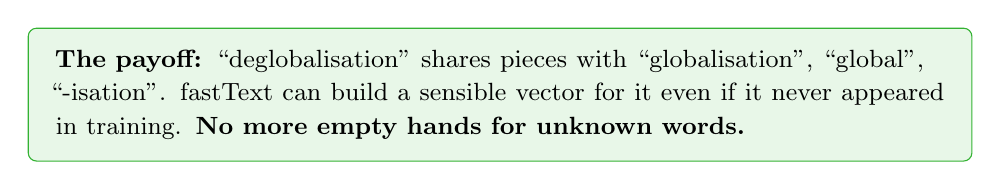
\begin{tikzpicture}
  \node[fill=lightgreen, draw=wurgreen, rounded corners=3pt,
        inner xsep=10pt, inner ysep=8pt, text width=\textwidth-24pt]{%
    {\small \textbf{The payoff:} ``deglobalisation'' shares pieces with ``globalisation'',
    ``global'', ``-isation''. fastText can build a sensible vector for it even if it never
    appeared in training. \textbf{No more empty hands for unknown words.}}};
\end{tikzpicture}
\end{frame}

% ── SLIDE 3: when to use ──────────────────────────────────────────────────
\begin{frame}{When Does This Matter?}
\vspace{0.3cm}
\begin{columns}[T]
  \column{0.48\textwidth}
  \vspace{0pt}
  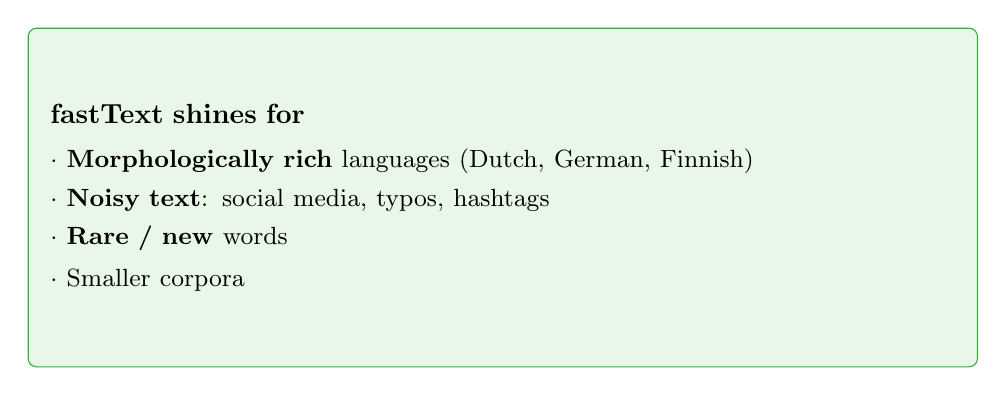
\begin{tikzpicture}
    \node[fill=lightgreen, draw=wurgreen, rounded corners=3pt,
          inner xsep=8pt, inner ysep=8pt, text width=\columnwidth-18pt, minimum height=4.3cm]{%
      \textbf{fastText shines for}\\[5pt]
      {\small
      $\cdot$ \textbf{Morphologically rich} languages (Dutch, German, Finnish)\\[3pt]
      $\cdot$ \textbf{Noisy text}: social media, typos, hashtags\\[3pt]
      $\cdot$ \textbf{Rare / new} words\\[3pt]
      $\cdot$ Smaller corpora}};
  \end{tikzpicture}

  \column{0.48\textwidth}
  \vspace{0pt}
  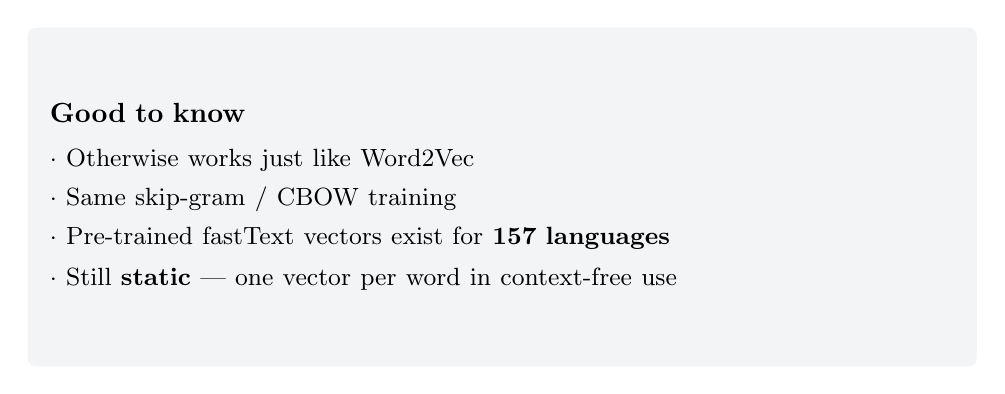
\begin{tikzpicture}
    \node[fill=lightgray, rounded corners=3pt,
          inner xsep=8pt, inner ysep=8pt, text width=\columnwidth-18pt, minimum height=4.3cm]{%
      \textbf{Good to know}\\[5pt]
      {\small
      $\cdot$ Otherwise works just like Word2Vec\\[3pt]
      $\cdot$ Same skip-gram / CBOW training\\[3pt]
      $\cdot$ Pre-trained fastText vectors exist for \textbf{157 languages}\\[3pt]
      $\cdot$ Still \textbf{static} --- one vector per word in context-free use}};
  \end{tikzpicture}
\end{columns}

\medskip
{\small\textcolor{midgray}{\textit{For a Dutch-language or social-media corpus, fastText is
often a better default than plain Word2Vec or GloVe.}}}
\end{frame}

% ── SLIDE 4: recap ────────────────────────────────────────────────────────
\begin{frame}{Takeaway}
\vspace{0.4cm}
\begin{itemize}\setlength\itemsep{10pt}
  \item[\textcolor{wurgreen}{\faCheck}]
    Plain static embeddings \textbf{drop words they never saw} (the OOV problem)
  \item[\textcolor{wurgreen}{\faCheck}]
    \textbf{fastText} represents words as \textbf{subword pieces}, so it can build vectors for
    unseen words
  \item[\textcolor{wurgreen}{\faCheck}]
    Especially useful for \textbf{morphologically rich languages} and \textbf{noisy text}
  \item[\textcolor{wurgreen}{\faCheck}]
    It is still a \textbf{static} embedding --- it does not solve the \emph{context} problem
    (``bank'' still gets one vector)
\end{itemize}

\medskip
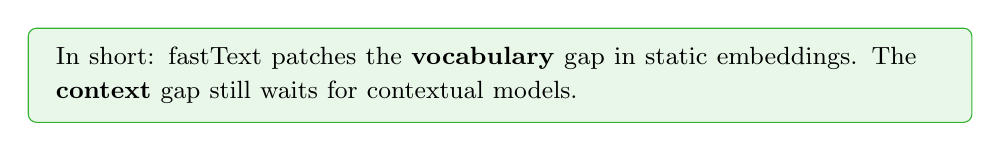
\begin{tikzpicture}
  \node[fill=lightgreen, draw=wurgreen, rounded corners=3pt,
        inner xsep=10pt, inner ysep=7pt, text width=\textwidth-24pt]{%
    {\small In short: fastText patches the \textbf{vocabulary} gap in static embeddings.
    The \textbf{context} gap still waits for contextual models.}};
\end{tikzpicture}
\end{frame}


% ═══════════════════════════════════════════════════════════════════════
% PART 2: EMBEDDINGS AS FEATURES FOR CLASSIFICATION
% ═══════════════════════════════════════════════════════════════════════

% ── SLIDE 1: connect back ─────────────────────────────────────────────────
\begin{frame}{Bringing It Full Circle}
\vspace{0.2cm}
{\small On Day 1 we built \textbf{supervised classifiers} on top of a \textbf{bag-of-words /
TF-IDF} matrix. Now we have a richer representation --- \textbf{embeddings}. Can we swap one
in for the other?}

\medskip
\begin{center}
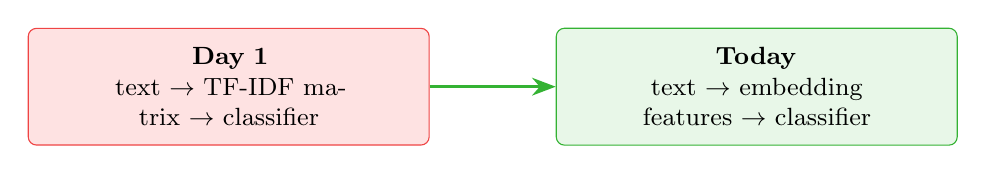
\begin{tikzpicture}[font=\small, node distance=0.8cm]
  \node[fill=warnred, draw=warnborder, rounded corners=3pt, inner sep=7pt, text width=4.6cm, align=center] (bow)
    {\textbf{Day 1}\\ text $\rightarrow$ TF-IDF matrix $\rightarrow$ classifier};
  \node[fill=lightgreen, draw=wurgreen, rounded corners=3pt, inner sep=7pt,
        text width=4.6cm, align=center, right=1.6cm of bow] (emb)
    {\textbf{Today}\\ text $\rightarrow$ embedding features $\rightarrow$ classifier};
  \draw[-{Stealth[length=3mm]}, wurgreen, line width=1.2pt] (bow) -- (emb);
\end{tikzpicture}
\end{center}

\bigskip
{\small The classifier stays the same (logistic regression, say). All that changes is
\textbf{how we turn each document into numbers}. This is the payoff of everything we have
learned about embeddings.}
\end{frame}

% ── SLIDE 2: document vector ──────────────────────────────────────────────
\begin{frame}{From Word Vectors to a Document Vector}
\vspace{0.2cm}
{\small A classifier needs \textbf{one vector per document}. Embeddings give us one vector per
\textbf{word}. The simplest bridge (from earlier): \textbf{average} the word vectors.}

\medskip
\begin{center}
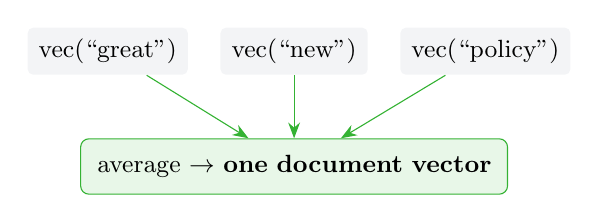
\begin{tikzpicture}[font=\small, node distance=0.5cm]
  \node (w1) [fill=lightgray, rounded corners=2pt, inner sep=4pt] {vec(``great'')};
  \node (w2) [fill=lightgray, rounded corners=2pt, inner sep=4pt, right=0.4cm of w1] {vec(``new'')};
  \node (w3) [fill=lightgray, rounded corners=2pt, inner sep=4pt, right=0.4cm of w2] {vec(``policy'')};
  \node (avg) [fill=lightgreen, draw=wurgreen, rounded corners=3pt, inner sep=6pt,
        below=0.8cm of w2, text width=5cm, align=center] {average $\rightarrow$ \textbf{one document vector}};
  \draw[-{Stealth[length=2mm]}, wurgreen] (w1) -- (avg);
  \draw[-{Stealth[length=2mm]}, wurgreen] (w2) -- (avg);
  \draw[-{Stealth[length=2mm]}, wurgreen] (w3) -- (avg);
\end{tikzpicture}
\end{center}

\medskip
{\small Each document becomes a single dense vector (say 300 numbers) --- ready to feed into
exactly the same classifiers as Day 1. Optionally weight the average by \textbf{TF-IDF} so
distinctive words count more.}
\end{frame}

% ── SLIDE 3: BoW vs embeddings tradeoffs ──────────────────────────────────
\begin{frame}{Embeddings vs.\ Bag-of-Words as Features}
\vspace{0.3cm}
\begin{columns}[T]
  \column{0.48\textwidth}
  \vspace{0pt}
  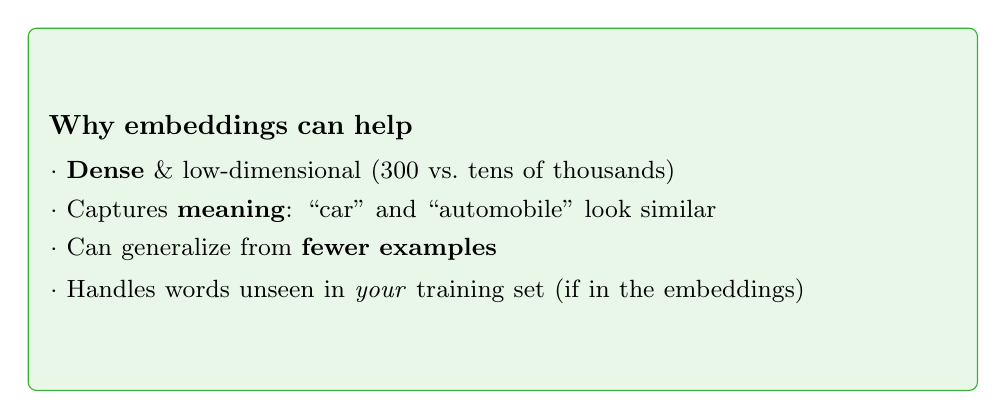
\begin{tikzpicture}
    \node[fill=lightgreen, draw=wurgreen, rounded corners=3pt,
          inner xsep=8pt, inner ysep=8pt, text width=\columnwidth-18pt, minimum height=4.6cm]{%
      \textbf{Why embeddings can help}\\[5pt]
      {\small
      $\cdot$ \textbf{Dense} \& low-dimensional (300 vs.\ tens of thousands)\\[3pt]
      $\cdot$ Captures \textbf{meaning}: ``car'' and ``automobile'' look similar\\[3pt]
      $\cdot$ Can generalize from \textbf{fewer examples}\\[3pt]
      $\cdot$ Handles words unseen in \emph{your} training set (if in the embeddings)}};
  \end{tikzpicture}

  \column{0.48\textwidth}
  \vspace{0pt}
  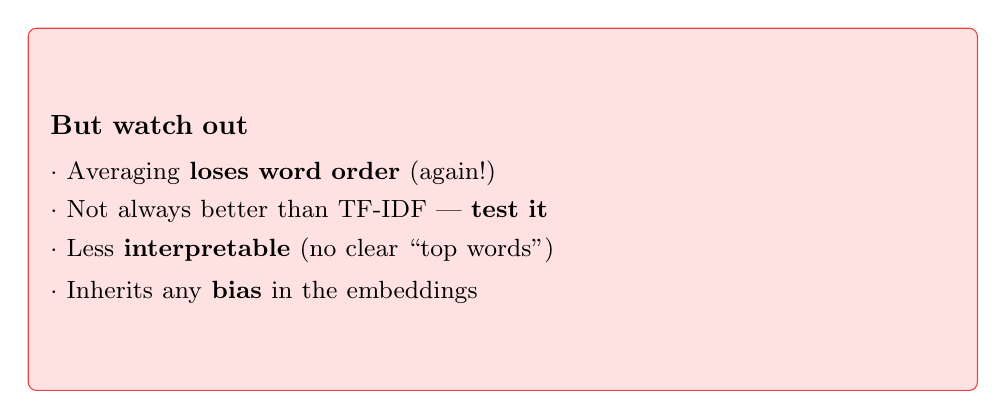
\begin{tikzpicture}
    \node[fill=warnred, draw=warnborder, rounded corners=3pt,
          inner xsep=8pt, inner ysep=8pt, text width=\columnwidth-18pt, minimum height=4.6cm]{%
      \textbf{But watch out}\\[5pt]
      {\small
      $\cdot$ Averaging \textbf{loses word order} (again!)\\[3pt]
      $\cdot$ Not always better than TF-IDF --- \textbf{test it}\\[3pt]
      $\cdot$ Less \textbf{interpretable} (no clear ``top words'')\\[3pt]
      $\cdot$ Inherits any \textbf{bias} in the embeddings}};
  \end{tikzpicture}
\end{columns}

\medskip
{\small\textcolor{midgray}{\textit{On short, clean text TF-IDF is a very strong baseline.
Embeddings tend to win when meaning and generalization matter most.}}}
\end{frame}

% ── SLIDE 4: to the notebook / recap ──────────────────────────────────────
\begin{frame}{Takeaway}
\vspace{0.4cm}
\begin{itemize}\setlength\itemsep{10pt}
  \item[\textcolor{wurgreen}{\faCheck}]
    Embeddings can replace \textbf{TF-IDF as the features} feeding a classifier
  \item[\textcolor{wurgreen}{\faCheck}]
    Turn each document into one vector by \textbf{averaging} its word vectors
    (optionally TF-IDF weighted)
  \item[\textcolor{wurgreen}{\faCheck}]
    Upsides: dense, meaning-aware, generalizes from less data
  \item[\textcolor{wurgreen}{\faCheck}]
    Downsides: loses order, less interpretable, and \textbf{not automatically better} ---
    always compare against the TF-IDF baseline
\end{itemize}

\medskip
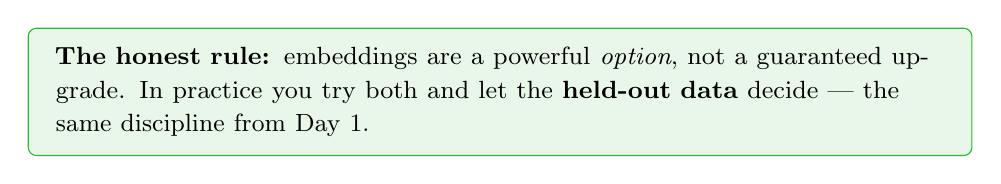
\begin{tikzpicture}
  \node[fill=lightgreen, draw=wurgreen, rounded corners=3pt,
        inner xsep=10pt, inner ysep=7pt, text width=\textwidth-24pt]{%
    {\small \textbf{The honest rule:} embeddings are a powerful \emph{option}, not a
    guaranteed upgrade. In practice you try both and let the \textbf{held-out data} decide ---
    the same discipline from Day 1.}};
\end{tikzpicture}
\end{frame}

\end{document}
